\documentclass{article}

\usepackage[utf8]{inputenc}
\usepackage[
    a4paper, top=2.5cm, bottom=2.5cm, left=2cm, right=2.5cm
]{geometry}
\usepackage{graphicx}
\usepackage{minted}
\usepackage{xeCJK}

\setCJKmainfont{Noto Sans CJK TC}
\setmainfont{Noto Sans CJK TC}

\setlength{\parindent}{0cm}
\renewcommand{\baselinestretch}{1.5}

\begin{document}

\section*{Module Explanation}

\begin{enumerate}
    \item[1.] cache controller

        在\mintinline{text}{dcache_controller.v},它會存自己的state,在每個
        cycle改變state並設定\mintinline{text}{mem_enable}、

        \mintinline{text}{mem_write}、\mintinline{text}{cache_write}和
        \mintinline{text}{wtite_back}四個變數,同時決定下一個state。這四個變數會決定
        cache controller要傳給data memory和cache的東西。假設cache回傳hit的話,就可以
        直接在\mintinline{text}{r_hit_data}和\mintinline{text}{w_hit_data}上操作
        ,等到cache miss的時候再把寫過的data傳回去data memory。可以參考以下的FSM。

        \begin{figure}[h]
            \centering
            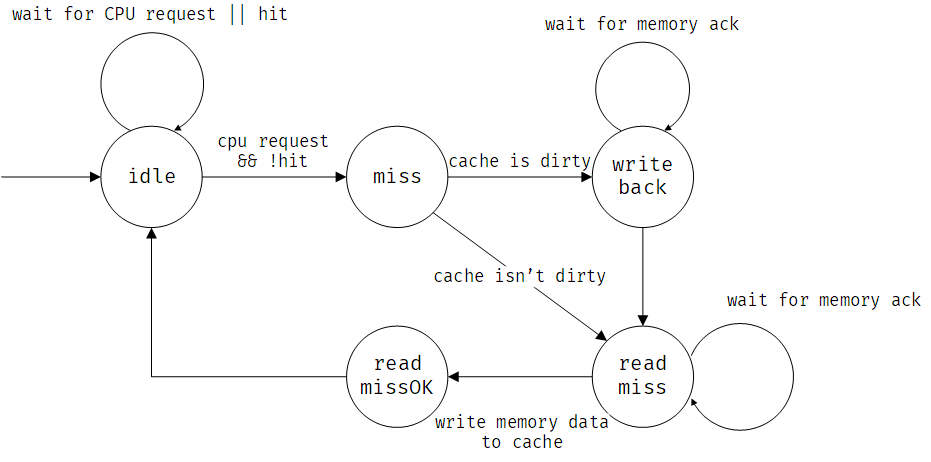
\includegraphics[width=\textwidth]{1.png}
        \end{figure}

    \item[2.] cache sram

        在\mintinline{text}{dcache_sram.v},接在cache controller上,它用LRU的方式
        存cache。它會先檢查\mintinline{text}{tag_i}是否在cache裡面且是valid的,並輸出
        對應的\mintinline{text}{data_o}。LRU的實作方法是用一個陣列存上次read的是0還是1
        ,並依此決定要把哪個換掉。

    \item[3.] CPU

        基於上次lab的CPU做修改,主要是把上次的data memory換成cache controller,
        然後把MemStall訊號接到各個pipeline register和PC上,以及把要給data memory
        的訊號接到cache controller上。

    \item[4.] other

        都是從lab1直接搬過來,然後做一些小修改。在4個pipeline register加上MemStall這個
        input,用來在cache read/write miss時stall。把上次的ALU的input加上signed,原
        因在Difficulties Encountered那邊。
\end{enumerate}

\pagebreak

\section*{Difficulties Encountered and Solutions in This Lab}

\begin{enumerate}
    \item[1.] ALU的srai寫錯,一直錯第二個測資,後來發現是沒有加signed。
    \item[2.] cache controller裡的\mintinline{text}{r_hit_data}和
        \mintinline{text}{w_hit_data}陣列取值原本是寫
        \mintinline{c}{(cpu_offset >> 2) << 5},結果會錯。後來才發現這樣寫
        不管怎樣取的都是0的位子,因為\mintinline{text}{cpu_offset}只有5個bit,
        後面的shift 5改成乘以32就可以了。
    \item[3.] 在測試最後的cache flush會把data memory歸零,後來在testbench
        加入判定tag valid就好了。
\end{enumerate}

\section*{Development Environment}

\begin{itemize}
    \item ArchWSL 21.8.28.0 @ windows 11 professional 21h2 22000.434
    \item Linux kernel version: 5.10.60.1-microsoft-standard-WSL2
    \item iverilog version: 11.0 (stable)
    \item gtkwave version: 3.3.111
\end{itemize}

\begin{figure}[h]
  \centering
  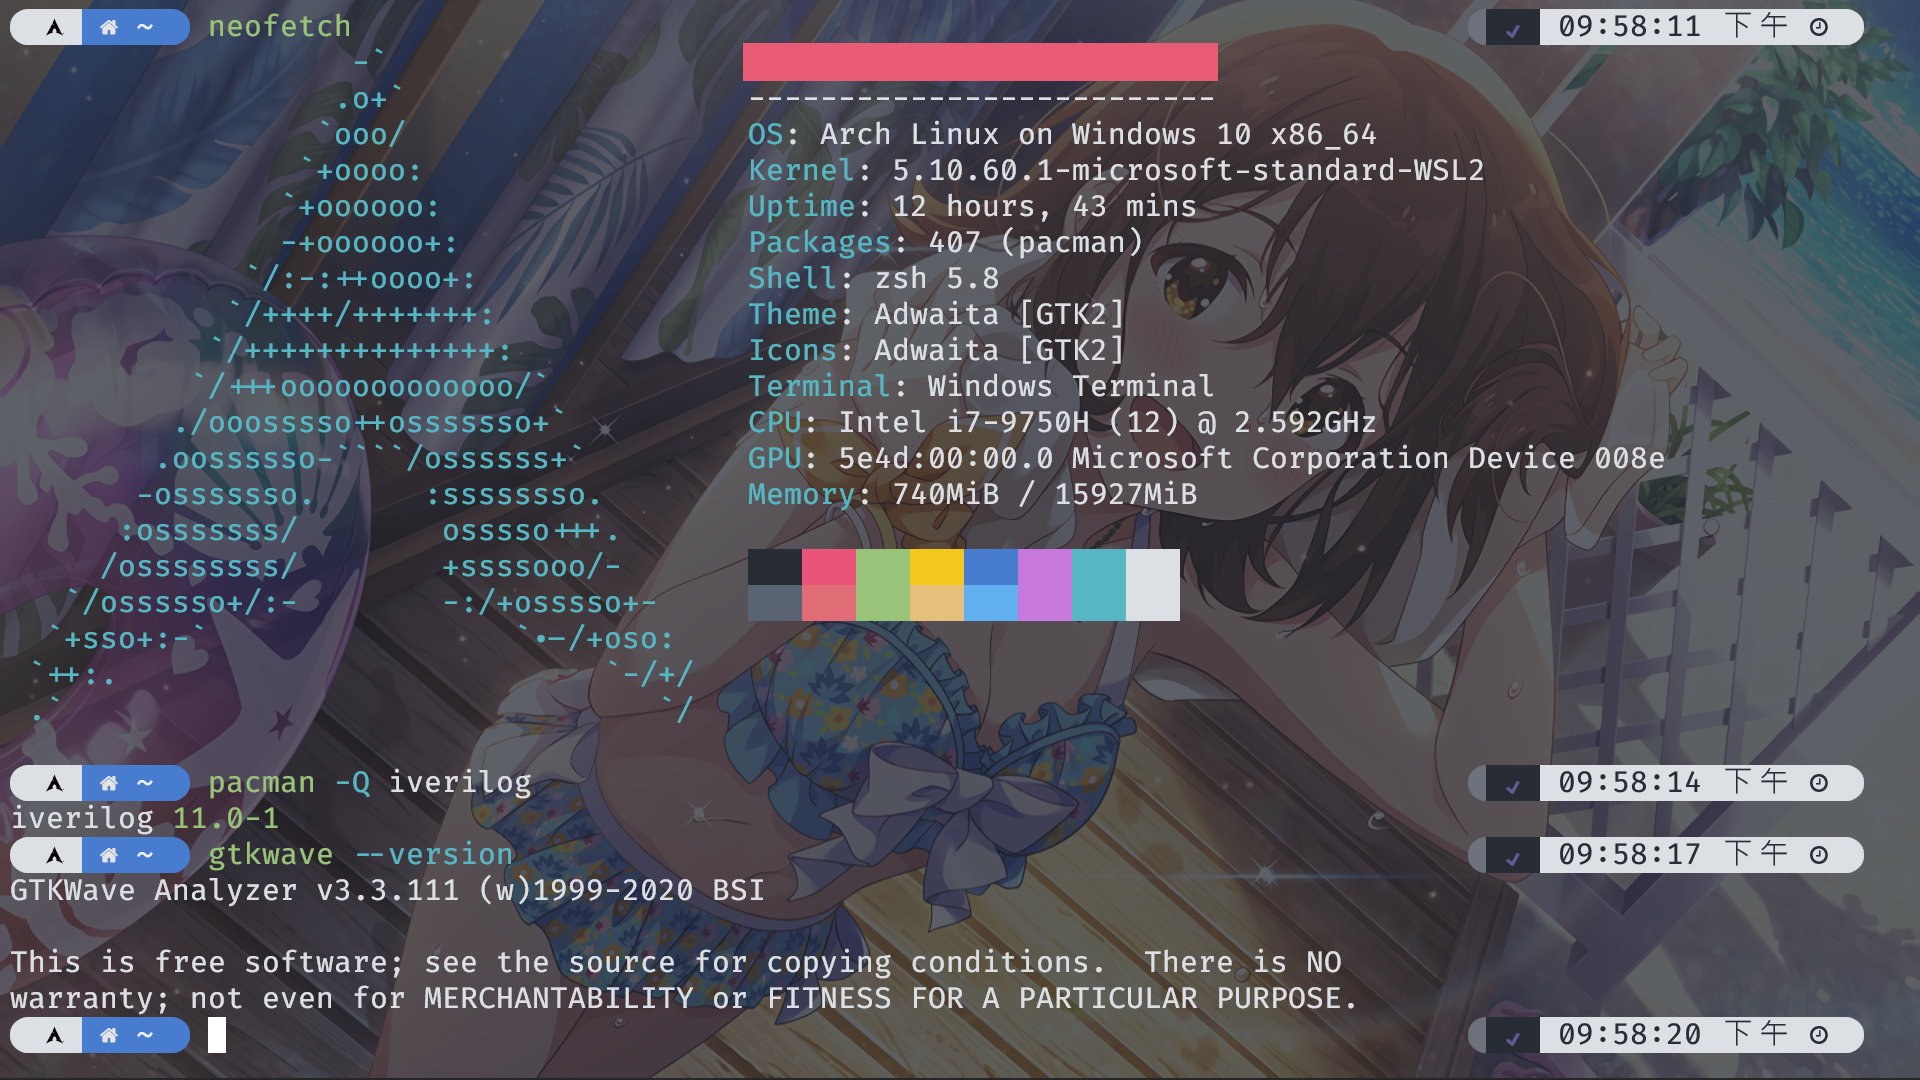
\includegraphics[width=\textwidth]{2.png}
\end{figure}

\end{document}
